\begin{atiTask}[
  title = Gleichgewichtspunkte und kleine Schwingungen
]
  Eine Perle $P$ mit Masse $m$ soll sich reibungsfrei auf einem Reifen mit Mittelpunkt $M$ und Radius $R$ bewegen können.
  Sie steht dabei unter der Einwirkung sowohl der Schwerkraft als auch einer elastischen Kraft.
  Letztere wird von einer Feder mit Federkonstante $k$ ausgeübt, die im Punkt $F$ befestigt ist und im entspannten Zustand die Länge $l_0 = \frac{R}{2}$ hat.
  Die Position der Perle auf dem Reifen wird durch den Winkel $\theta(t)$ beschrieben.
  Die zugehörige Länge der gedehnten Feder ist $l(t)$.
  \begin{figure}[H]
    \center
    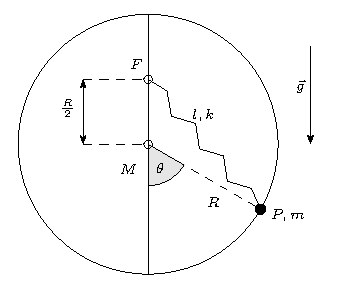
\includegraphics{task-gleichgewichtspunkte_und_kleine_schwingungen-sketch.pdf}
  \end{figure}
  Die gesamte Kraftkomponente, die die Perle auf dem Reifen bewegt, ist
  \[
    F = \boxb{-mg + \frac{Rk}{2}\curvb{1 - \frac{1}{\sqrt{5 + 4\cos \theta}}}}\sin \theta \ .
  \]
  \begin{atiSubtasks}
    \item{
      Bestimmen Sie alle Winkel $\theta$, die Gleichgewichtslagen der Perle beschreiben.
      Dabei ist es ausreichend, die Bestimmungsgleichungen für diese Winkel in impliziter Form anzugeben.
    }
    \item{
      Entscheiden Sie über die Stabilität dieser Gleichgewichtslagen.

      \begin{atiNote}
        Für Fallunterscheidungen ist es zweckmäßig, den dimensionalen Parameter
        \[
          \kappa = \frac{k}{k_\m{krit}} \quad \text{mit} \quad k_\m{krit} = 3\frac{mg}{R}
        \]
        einzuführen.
      \end{atiNote}
    }
  \end{atiSubtasks}
\end{atiTask}